Continuando con el análisis de las mediciones de un multimetro true RMS, en este experimento se busca comparar nuevamente los valores dados por este multimetro en comparación con uno que brinda el valor medio de la señal, para ello se procedió a medir la forma de onda proveniente de un circuito con control de ángulo de conducción, el cual se puede observar en la figura \ref{fig:circ_triac}




\begin{figure}[H]
    \centering
    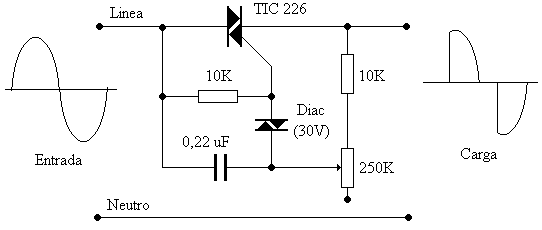
\includegraphics[width=0.8\linewidth]{Imagenes/circ_triac.png}
    \caption{Circuito Experimento 4: Control de ángulo de conducción}
    \label{fig:circ_triac}
\end{figure}

Este circuito se conecto a la tensión de linea y se procedió a conectar los multimetros y el osciloscopio, utilizando siempre el transformador de aislación para evitar inconvenientes que causen daños a los instrumentos. En la figura \ref{fig:conec_exp4}se observa la conexión correcta para realizar la experimentación. 
\begin{figure}[H]
    \centering
    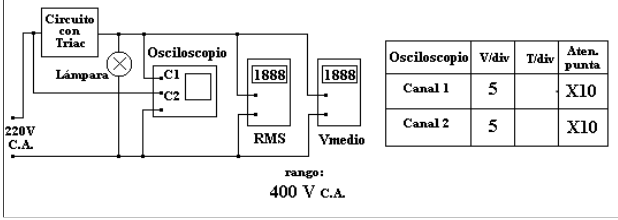
\includegraphics[width=0.6\linewidth,trim= 5pt 5pt 8.5cm 0,clip]{Imagenes/conec_exp4.png}
    \caption{Conexión Experimento 4}
    \label{fig:conec_exp4}
\end{figure}

\begin{table}[H]
    \centering
    \scalebox{1}{
    \begin{tabular}{|c|c|c|c|c|}
    \hline
         V/div (C. Y1) & V/div (C.Y2) & t/div & Aten. Y1 & Aten. Y2 \\
    \hline
         5 $V$ & 5 $V$ &  $ms$ & x10 & x10\\
    \hline
    \end{tabular}}
        %\def\tablename{Tabla} 
        \caption{Configuración del Osciloscopio}
        \label{tab:cont4}
\end{table}
Como primer paso se midió la tensión de entrada al circuito, obteniendo el siguiente valor.

\begin{equation*}
    V_i = 230.8 ~[V]
\end{equation*}

Luego a través del potenciómetro que viene incluido en el circuito de control, se fue variando el ángulo de conducción y a su vez se fue midiendo los valores de tensión que había a la salida del circuito. Se variaron los ángulos de salida según las siguientes gráficas, y se espera obtener formas de onda similares en las mediciones.

\begin{figure}[H]
    \centering
    \begin{minipage}{0.49\textwidth}
        \centering
        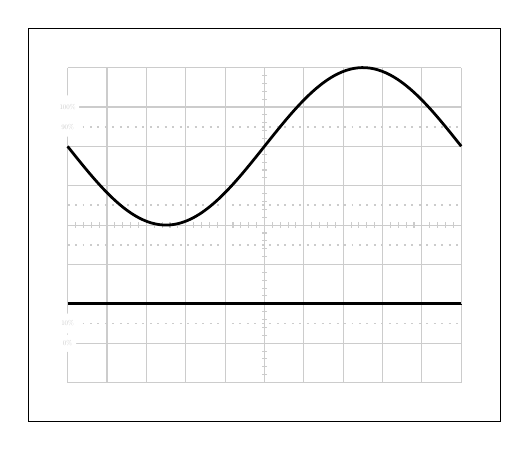
\begin{tikzpicture}[scale=0.5,every node/.style={transform shape}]
\def\angC{180}
    %Lineas intermedias grilla
    \foreach \x in {-5,-4.8,...,4.8,5}{
        \draw[gray!40,thin,shift={(\x,0)}] (0pt,2pt) -- (0pt,-2pt);
    }
    \foreach \y in {-4,-3.8,...,3.8,4}{
        \draw[gray!40,thin,shift={(0,\y)}] (2pt,0pt) -- (-2pt,0pt);
    }
    \foreach \a [evaluate={\y=\a*0.5}] in {-5,-1,1,5}{
        \draw[gray!40,line width=0.7pt,dotted] (-5,\y) -- (5,\y);
    }

    %Grilla
    \draw[thin,gray!40] (-5,-4) grid (5,4);
    \node[fill=white,text=gray!40,circle,scale=0.5] at (-5,3) {$100\%$};
    \node[fill=white,text=gray!40,circle,scale=0.5] at (-5,2.5) {$90\%$};
    \node[fill=white,text=gray!40,circle,scale=0.5] at (-5,-2.5) {$10\%$};
    \node[fill=white,text=gray!40,circle,scale=0.5] at (-5,-3) {$0\%$};
    \draw[black] (-6,-5) rectangle(6,5);
    
    
    \draw [line width=1pt,black] plot[smooth,samples=100,domain=-5:5](\x,{2*sin(deg(\x*pi*0.2))+2});

    
    \draw [thin,black] plot[smooth,samples=100,domain=\angC/36:5](\x,{2*sin(deg(\x*pi*0.2))-2});
    \draw [thin,black] plot[smooth,samples=100,domain=-5+\angC/36:0](\x,{2*sin(deg(\x*pi*0.2))-2});
    \draw[thin,black](\angC/36,{2*sin(deg(3.14*\angC/36*0.2))-2})--(\angC/36,-2);
    \draw[thin,black](-5+\angC/36,{2*sin(deg(3.14*(-5+\angC/36)*0.2))-2})--(-5+\angC/36,-2);
    \draw[line width=1pt,black](-5,-2)--(-5+\angC/36,-2) (0,-2)--(\angC/36,-2);
\end{tikzpicture}
\caption*{$Ang_{cond}=0$}
    \end{minipage}
    \begin{minipage}{0.49\textwidth}
        \centering
        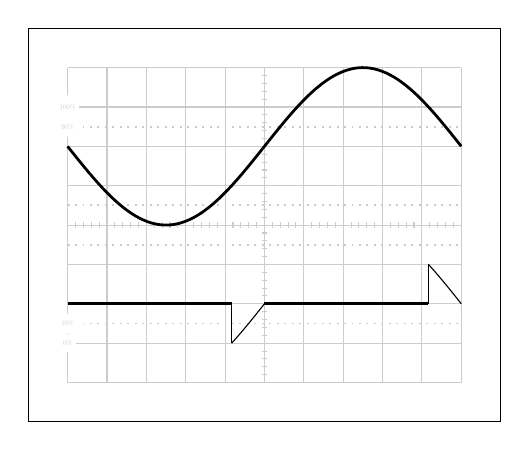
\begin{tikzpicture}[scale=0.5,every node/.style={transform shape}]
\def\angC{150}
    %Lineas intermedias grilla
    \foreach \x in {-5,-4.8,...,4.8,5}{
        \draw[gray!40,thin,shift={(\x,0)}] (0pt,2pt) -- (0pt,-2pt);
    }
    \foreach \y in {-4,-3.8,...,3.8,4}{
        \draw[gray!40,thin,shift={(0,\y)}] (2pt,0pt) -- (-2pt,0pt);
    }
    \foreach \a [evaluate={\y=\a*0.5}] in {-5,-1,1,5}{
        \draw[gray!40,line width=0.7pt,dotted] (-5,\y) -- (5,\y);
    }

    %Grilla
    \draw[thin,gray!40] (-5,-4) grid (5,4);
    \node[fill=white,text=gray!40,circle,scale=0.5] at (-5,3) {$100\%$};
    \node[fill=white,text=gray!40,circle,scale=0.5] at (-5,2.5) {$90\%$};
    \node[fill=white,text=gray!40,circle,scale=0.5] at (-5,-2.5) {$10\%$};
    \node[fill=white,text=gray!40,circle,scale=0.5] at (-5,-3) {$0\%$};
    \draw[black] (-6,-5) rectangle(6,5);
    
    
    \draw [line width=1pt,black] plot[smooth,samples=100,domain=-5:5](\x,{2*sin(deg(\x*pi*0.2))+2});

    \draw [thin,black] plot[smooth,samples=100,domain=\angC/36:5](\x,{2*sin(deg(\x*pi*0.2))-2});
    \draw [thin,black] plot[smooth,samples=100,domain=-5+\angC/36:0](\x,{2*sin(deg(\x*pi*0.2))-2});
    \draw[thin,black](\angC/36,{2*sin(deg(3.14*\angC/36*0.2))-2})--(\angC/36,-2);
    \draw[thin,black](-5+\angC/36,{2*sin(deg(3.14*(-5+\angC/36)*0.2))-2})--(-5+\angC/36,-2);
    \draw[line width=1pt,black](-5,-2)--(-5+\angC/36,-2) (0,-2)--(\angC/36,-2);
\end{tikzpicture}
\caption*{$Ang_{cond}=30$}
    \end{minipage}
    \begin{minipage}{0.49\textwidth}
        \centering
        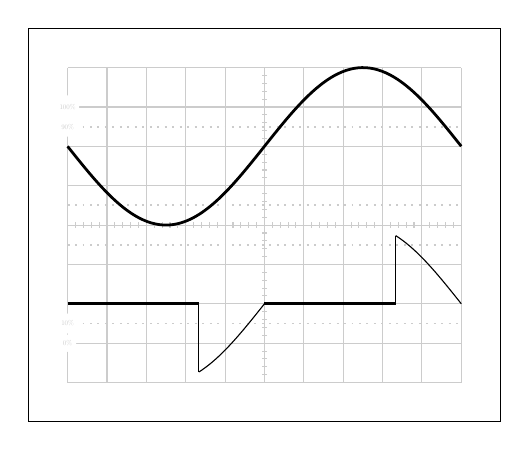
\begin{tikzpicture}[scale=0.5,every node/.style={transform shape}]
\def\angC{120}
    %Lineas intermedias grilla
    \foreach \x in {-5,-4.8,...,4.8,5}{
        \draw[gray!40,thin,shift={(\x,0)}] (0pt,2pt) -- (0pt,-2pt);
    }
    \foreach \y in {-4,-3.8,...,3.8,4}{
        \draw[gray!40,thin,shift={(0,\y)}] (2pt,0pt) -- (-2pt,0pt);
    }
    \foreach \a [evaluate={\y=\a*0.5}] in {-5,-1,1,5}{
        \draw[gray!40,line width=0.7pt,dotted] (-5,\y) -- (5,\y);
    }

    %Grilla
    \draw[thin,gray!40] (-5,-4) grid (5,4);
    \node[fill=white,text=gray!40,circle,scale=0.5] at (-5,3) {$100\%$};
    \node[fill=white,text=gray!40,circle,scale=0.5] at (-5,2.5) {$90\%$};
    \node[fill=white,text=gray!40,circle,scale=0.5] at (-5,-2.5) {$10\%$};
    \node[fill=white,text=gray!40,circle,scale=0.5] at (-5,-3) {$0\%$};
    \draw[black] (-6,-5) rectangle(6,5);
    
    
    \draw [line width=1pt,black] plot[smooth,samples=100,domain=-5:5](\x,{2*sin(deg(\x*pi*0.2))+2});

   
    \draw [thin,black] plot[smooth,samples=100,domain=\angC/36:5](\x,{2*sin(deg(\x*pi*0.2))-2});
    \draw [thin,black] plot[smooth,samples=100,domain=-5+\angC/36:0](\x,{2*sin(deg(\x*pi*0.2))-2});
    \draw[thin,black](\angC/36,{2*sin(deg(3.14*\angC/36*0.2))-2})--(\angC/36,-2);
    \draw[thin,black](-5+\angC/36,{2*sin(deg(3.14*(-5+\angC/36)*0.2))-2})--(-5+\angC/36,-2);
    \draw[line width=1pt,black](-5,-2)--(-5+\angC/36,-2) (0,-2)--(\angC/36,-2);
\end{tikzpicture}
\caption*{$Ang_{cond}=60$}
    \end{minipage}
    \centering
    \begin{minipage}{0.49\textwidth}
    \centering
        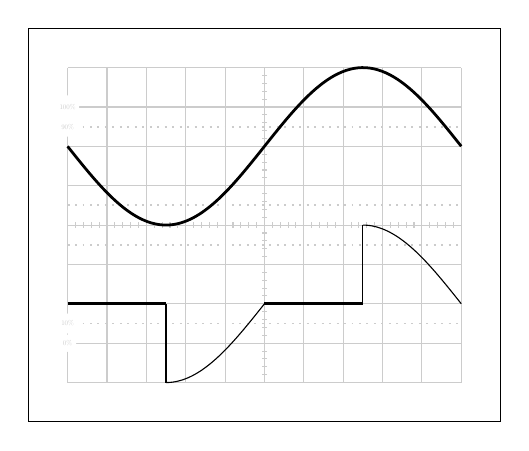
\begin{tikzpicture}[scale=0.5,every node/.style={transform shape}]
\def\angC{90}
    %Lineas intermedias grilla
    \foreach \x in {-5,-4.8,...,4.8,5}{
        \draw[gray!40,thin,shift={(\x,0)}] (0pt,2pt) -- (0pt,-2pt);
    }
    \foreach \y in {-4,-3.8,...,3.8,4}{
        \draw[gray!40,thin,shift={(0,\y)}] (2pt,0pt) -- (-2pt,0pt);
    }
    \foreach \a [evaluate={\y=\a*0.5}] in {-5,-1,1,5}{
        \draw[gray!40,line width=0.7pt,dotted] (-5,\y) -- (5,\y);
    }

    %Grilla
    \draw[thin,gray!40] (-5,-4) grid (5,4);
    \node[fill=white,text=gray!40,circle,scale=0.5] at (-5,3) {$100\%$};
    \node[fill=white,text=gray!40,circle,scale=0.5] at (-5,2.5) {$90\%$};
    \node[fill=white,text=gray!40,circle,scale=0.5] at (-5,-2.5) {$10\%$};
    \node[fill=white,text=gray!40,circle,scale=0.5] at (-5,-3) {$0\%$};
    \draw[black] (-6,-5) rectangle(6,5);
    
    
    \draw [line width=1pt,black] plot[smooth,samples=100,domain=-5:5](\x,{2*sin(deg(\x*pi*0.2))+2});

    \draw [thin,black] plot[smooth,samples=100,domain=\angC/36:5](\x,{2*sin(deg(\x*pi*0.2))-2});
    \draw [thin,black] plot[smooth,samples=100,domain=-5+\angC/36:0](\x,{2*sin(deg(\x*pi*0.2))-2});
    \draw[thin,black](\angC/36,{2*sin(deg(3.14*\angC/36*0.2))-2})--(\angC/36,-2);
    \draw[thin,black](-5+\angC/36,{2*sin(deg(3.14*(-5+\angC/36)*0.2))-2})--(-5+\angC/36,-2);
    \draw[line width=1pt,black](-5,-2)--(-5+\angC/36,-2) (0,-2)--(\angC/36,-2);
\end{tikzpicture}
\caption*{$Ang_{cond}=90$}
    \end{minipage}
    \begin{minipage}{0.49\textwidth}
    \centering
        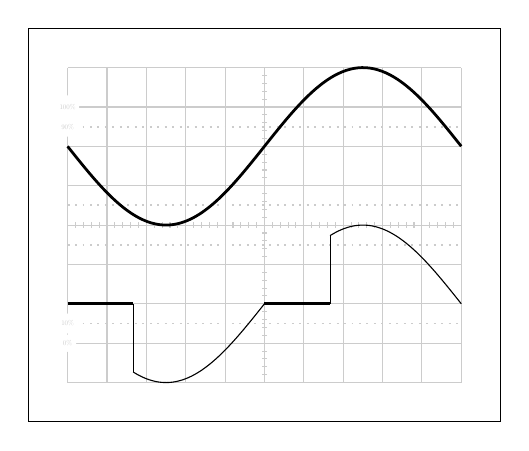
\begin{tikzpicture}[scale=0.5,every node/.style={transform shape}]
\def\angC{60}
    %Lineas intermedias grilla
    \foreach \x in {-5,-4.8,...,4.8,5}{
        \draw[gray!40,thin,shift={(\x,0)}] (0pt,2pt) -- (0pt,-2pt);
    }
    \foreach \y in {-4,-3.8,...,3.8,4}{
        \draw[gray!40,thin,shift={(0,\y)}] (2pt,0pt) -- (-2pt,0pt);
    }
    \foreach \a [evaluate={\y=\a*0.5}] in {-5,-1,1,5}{
        \draw[gray!40,line width=0.7pt,dotted] (-5,\y) -- (5,\y);
    }

    %Grilla
    \draw[thin,gray!40] (-5,-4) grid (5,4);
    \node[fill=white,text=gray!40,circle,scale=0.5] at (-5,3) {$100\%$};
    \node[fill=white,text=gray!40,circle,scale=0.5] at (-5,2.5) {$90\%$};
    \node[fill=white,text=gray!40,circle,scale=0.5] at (-5,-2.5) {$10\%$};
    \node[fill=white,text=gray!40,circle,scale=0.5] at (-5,-3) {$0\%$};
    \draw[black] (-6,-5) rectangle(6,5);
    
    
    \draw [line width=1pt,black] plot[smooth,samples=100,domain=-5:5](\x,{2*sin(deg(\x*pi*0.2))+2});

    \draw [thin,black] plot[smooth,samples=100,domain=\angC/36:5](\x,{2*sin(deg(\x*pi*0.2))-2});
    \draw [thin,black] plot[smooth,samples=100,domain=-5+\angC/36:0](\x,{2*sin(deg(\x*pi*0.2))-2});
    \draw[thin,black](\angC/36,{2*sin(deg(3.14*\angC/36*0.2))-2})--(\angC/36,-2);
    \draw[thin,black](-5+\angC/36,{2*sin(deg(3.14*(-5+\angC/36)*0.2))-2})--(-5+\angC/36,-2);
    \draw[line width=1pt,black](-5,-2)--(-5+\angC/36,-2) (0,-2)--(\angC/36,-2);
\end{tikzpicture}
\caption*{$Ang_{cond}=120$}
    \end{minipage}
    \begin{minipage}{0.49\textwidth}
    \centering
        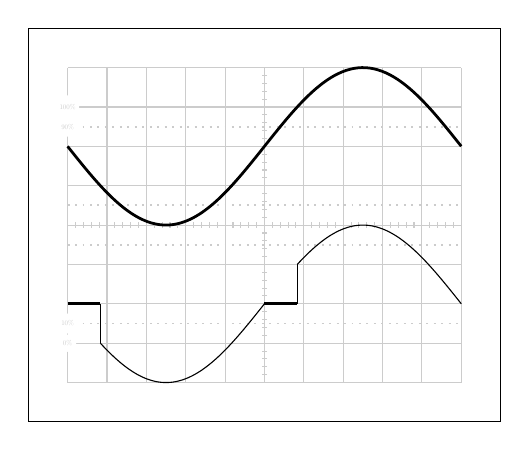
\begin{tikzpicture}[scale=0.5,every node/.style={transform shape}]
\def\angC{30}
    %Lineas intermedias grilla
    \foreach \x in {-5,-4.8,...,4.8,5}{
        \draw[gray!40,thin,shift={(\x,0)}] (0pt,2pt) -- (0pt,-2pt);
    }
    \foreach \y in {-4,-3.8,...,3.8,4}{
        \draw[gray!40,thin,shift={(0,\y)}] (2pt,0pt) -- (-2pt,0pt);
    }
    \foreach \a [evaluate={\y=\a*0.5}] in {-5,-1,1,5}{
        \draw[gray!40,line width=0.7pt,dotted] (-5,\y) -- (5,\y);
    }

    %Grilla
    \draw[thin,gray!40] (-5,-4) grid (5,4);
    \node[fill=white,text=gray!40,circle,scale=0.5] at (-5,3) {$100\%$};
    \node[fill=white,text=gray!40,circle,scale=0.5] at (-5,2.5) {$90\%$};
    \node[fill=white,text=gray!40,circle,scale=0.5] at (-5,-2.5) {$10\%$};
    \node[fill=white,text=gray!40,circle,scale=0.5] at (-5,-3) {$0\%$};
    \draw[black] (-6,-5) rectangle(6,5);
    
    
    \draw [line width=1pt,black] plot[smooth,samples=100,domain=-5:5](\x,{2*sin(deg(\x*pi*0.2))+2});

    \draw [thin,black] plot[smooth,samples=100,domain=\angC/36:5](\x,{2*sin(deg(\x*pi*0.2))-2});
    \draw [thin,black] plot[smooth,samples=100,domain=-5+\angC/36:0](\x,{2*sin(deg(\x*pi*0.2))-2});
    \draw[thin,black](\angC/36,{2*sin(deg(3.14*\angC/36*0.2))-2})--(\angC/36,-2);
    \draw[thin,black](-5+\angC/36,{2*sin(deg(3.14*(-5+\angC/36)*0.2))-2})--(-5+\angC/36,-2);
    \draw[line width=1pt,black](-5,-2)--(-5+\angC/36,-2) (0,-2)--(\angC/36,-2);
\end{tikzpicture}
\caption*{$Ang_{cond}=150$}
    \end{minipage}
\end{figure}


\unsubsubsection{Mediciones}

Estas mediciones fueron realizadas con los dos multímetros al mismo tiempo para así ir visualizando la diferencia entre los que media uno y lo que media el otro, obteniendo así la siguiente tabla de comparación.

\begin{table}[H]
    \centering
    \begin{tabular}{|c|c|c|c|c|c|c|c|}
    \hline
        \multirow{2}{*}{Fase} & $V_o$ (1) & $V_o$ (2) & \multirow{2}{*}{$\cfrac{V_{o_1}}{V_i}$} & \multirow{2}{*}{$\cfrac{V_{o_2}}{V_i}$} & Incertidumbre & Incertidumbre&Factor de\\
         & [V] & [V] &  &  & medición $V_{o_1}$ & medición $V_{o_2}$& corrección $\kappa$\\
        \hline
        0° & 0 & 0 & 0 & 0 & $\pm$0 & $\pm$0&0 \\ \hline
        30° & 43 & 17 & 0.186 & 0.074 & $\pm$0.37 & $\pm$0.51& 2.52 \\ \hline
        60° & 89 & 47 & 0.386 & 0.204 & $\pm$1.01 & $\pm$0.864&1.89 \\ \hline
        90° & 116 & 68 & 0.503 & 0.295 & $\pm$1.23 & $\pm$1.12& 1.70\\ \hline
        120° & 209 & 177 & 0.906 & 0.767 & $\pm$1.97 & $\pm$5.12& 1.18\\ \hline
        150° & 227 & 215 & 0.984 & 0.931 & $\pm$2.12 & $\pm$5.58& 1.05\\ \hline
        180° & 231 & 231 & 1 & 1 & $\pm$2.14 & $\pm$5.76& 1\\ \hline
    \end{tabular}
    \def\tablename{Tabla} 
    \caption{mediciones obtenidas}
    \label{tab:exp4}
\end{table}

A continuación en la figura \ref{fig:fot_exp4} se muestran las imágenes las formas de ondas visualizadas en el osciloscopio. Para poder observar dichas ondas completas en la pantalla fue necesario utilizar vernier de ganancia al máximo para atenuar las señales a un 30\% de su valor original.

\begin{figure}[H]
    \begin{center}
        \begin{subfigure}[b]{0.5\textwidth}
        \centering  
            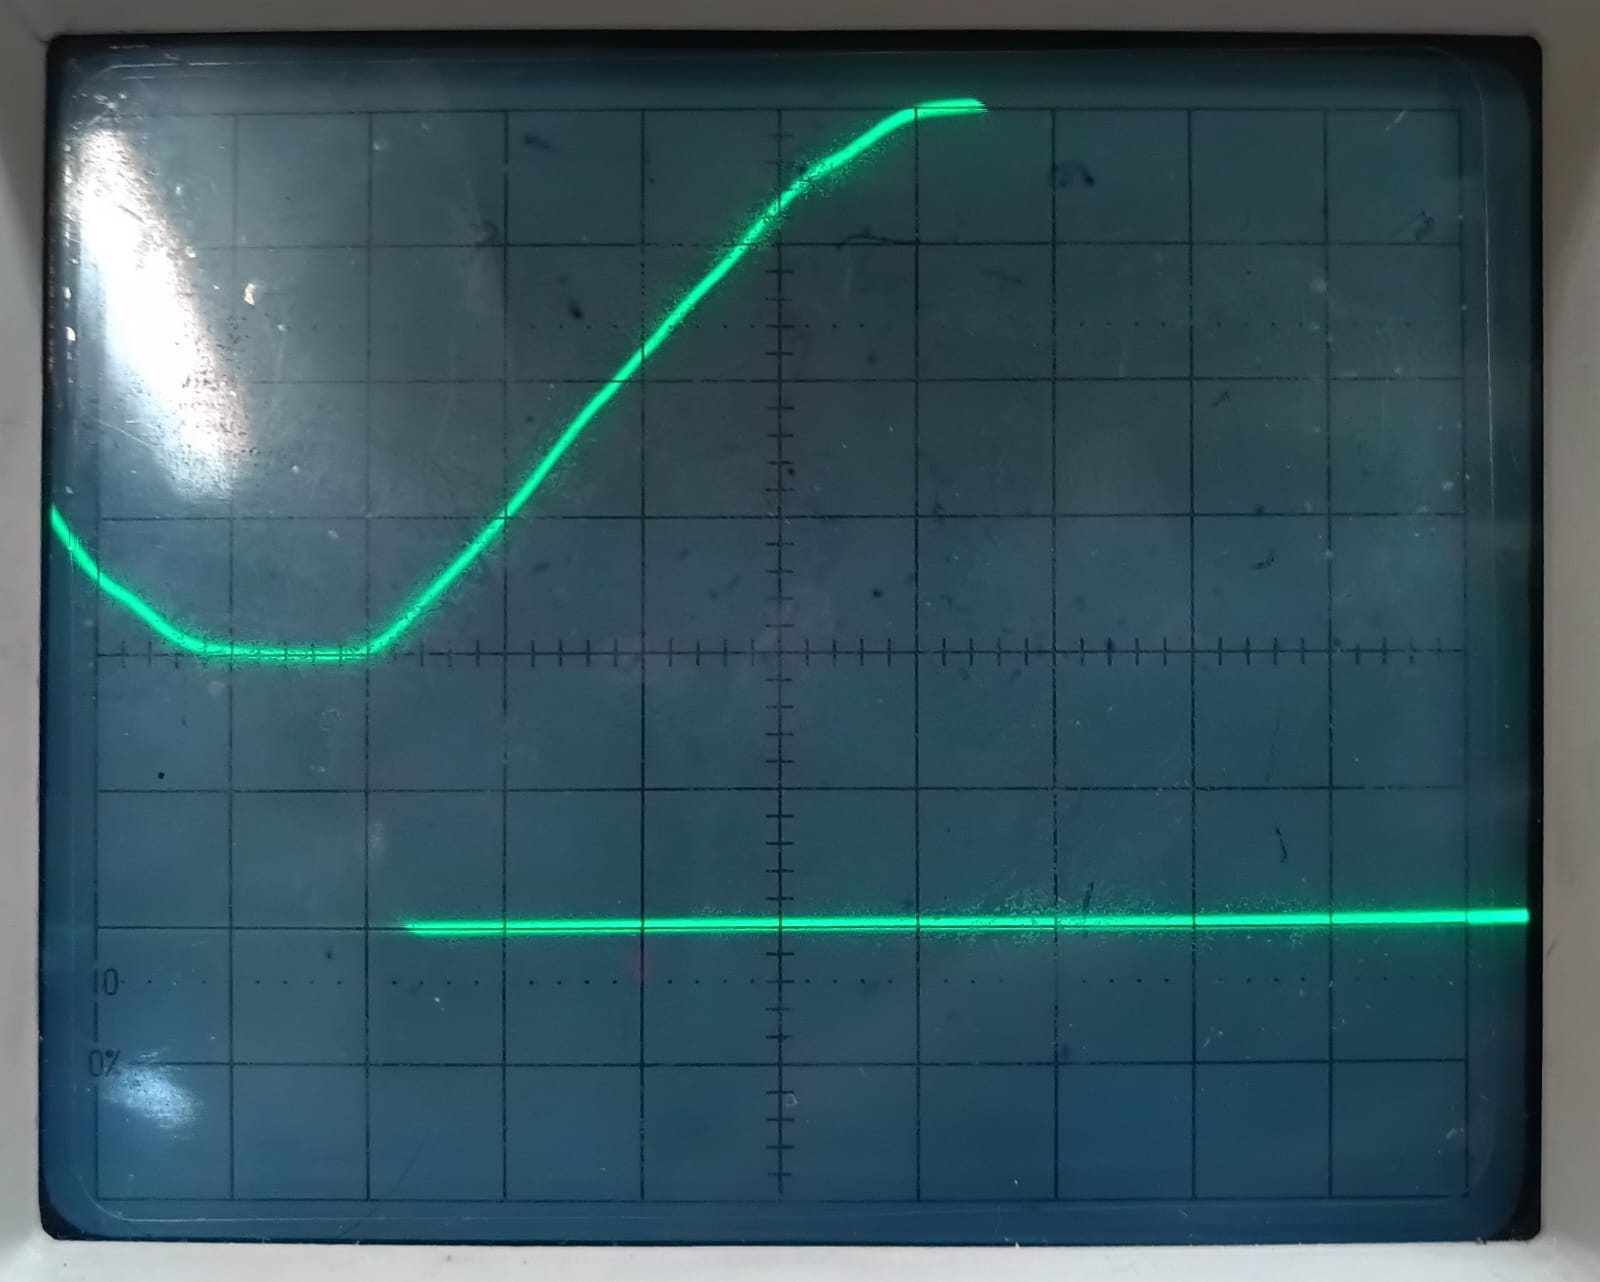
\includegraphics[width=0.65\textwidth]{Imagenes/0grad.jpeg}
        \label{}
        \caption{$Ang_{cond}=0$°}
    \end{subfigure}
    \hfill
        \begin{subfigure}[b]{0.49\textwidth}
        \centering  
            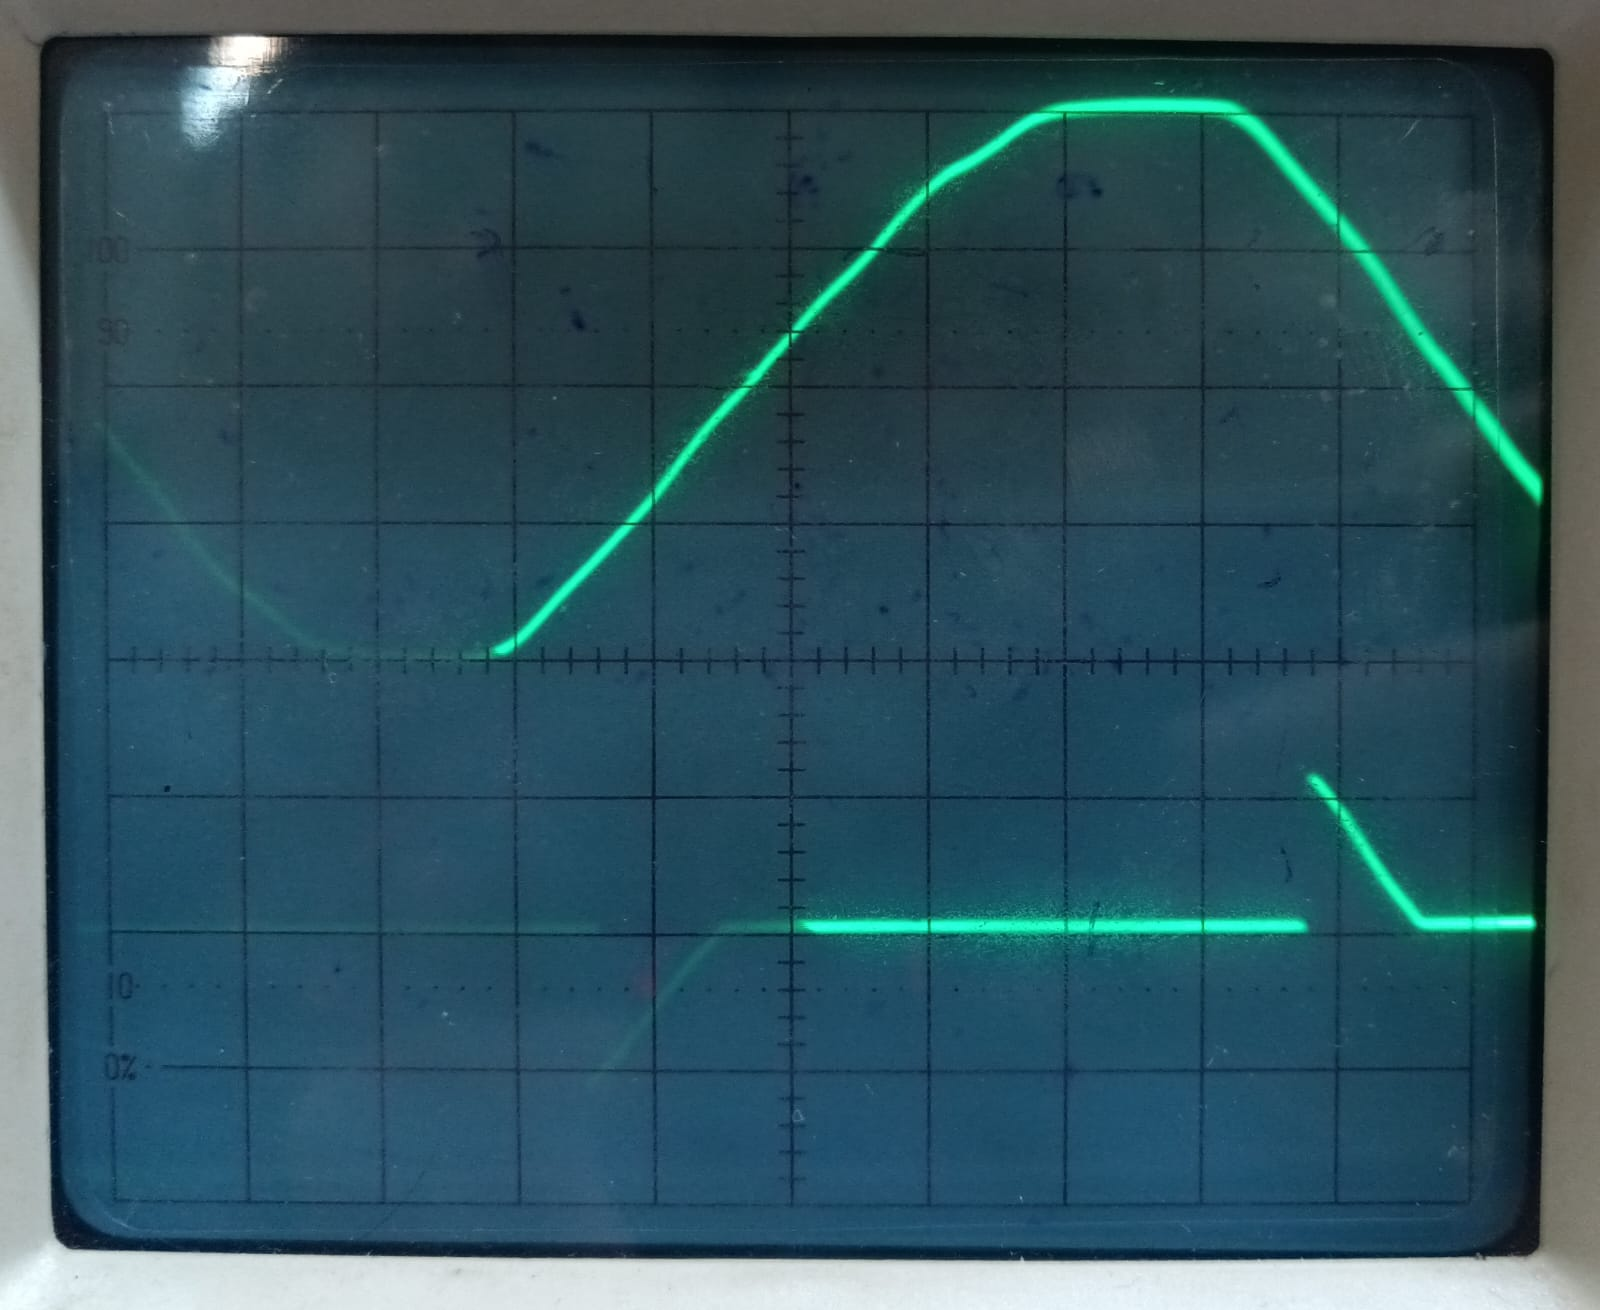
\includegraphics[width=0.65\textwidth]{Imagenes/30grad.jpeg}
        \label{}
        \caption{$Ang_{cond}=30$°}
    \end{subfigure}
    \hfill
        \begin{subfigure}[b]{0.5\textwidth}
        \centering  
            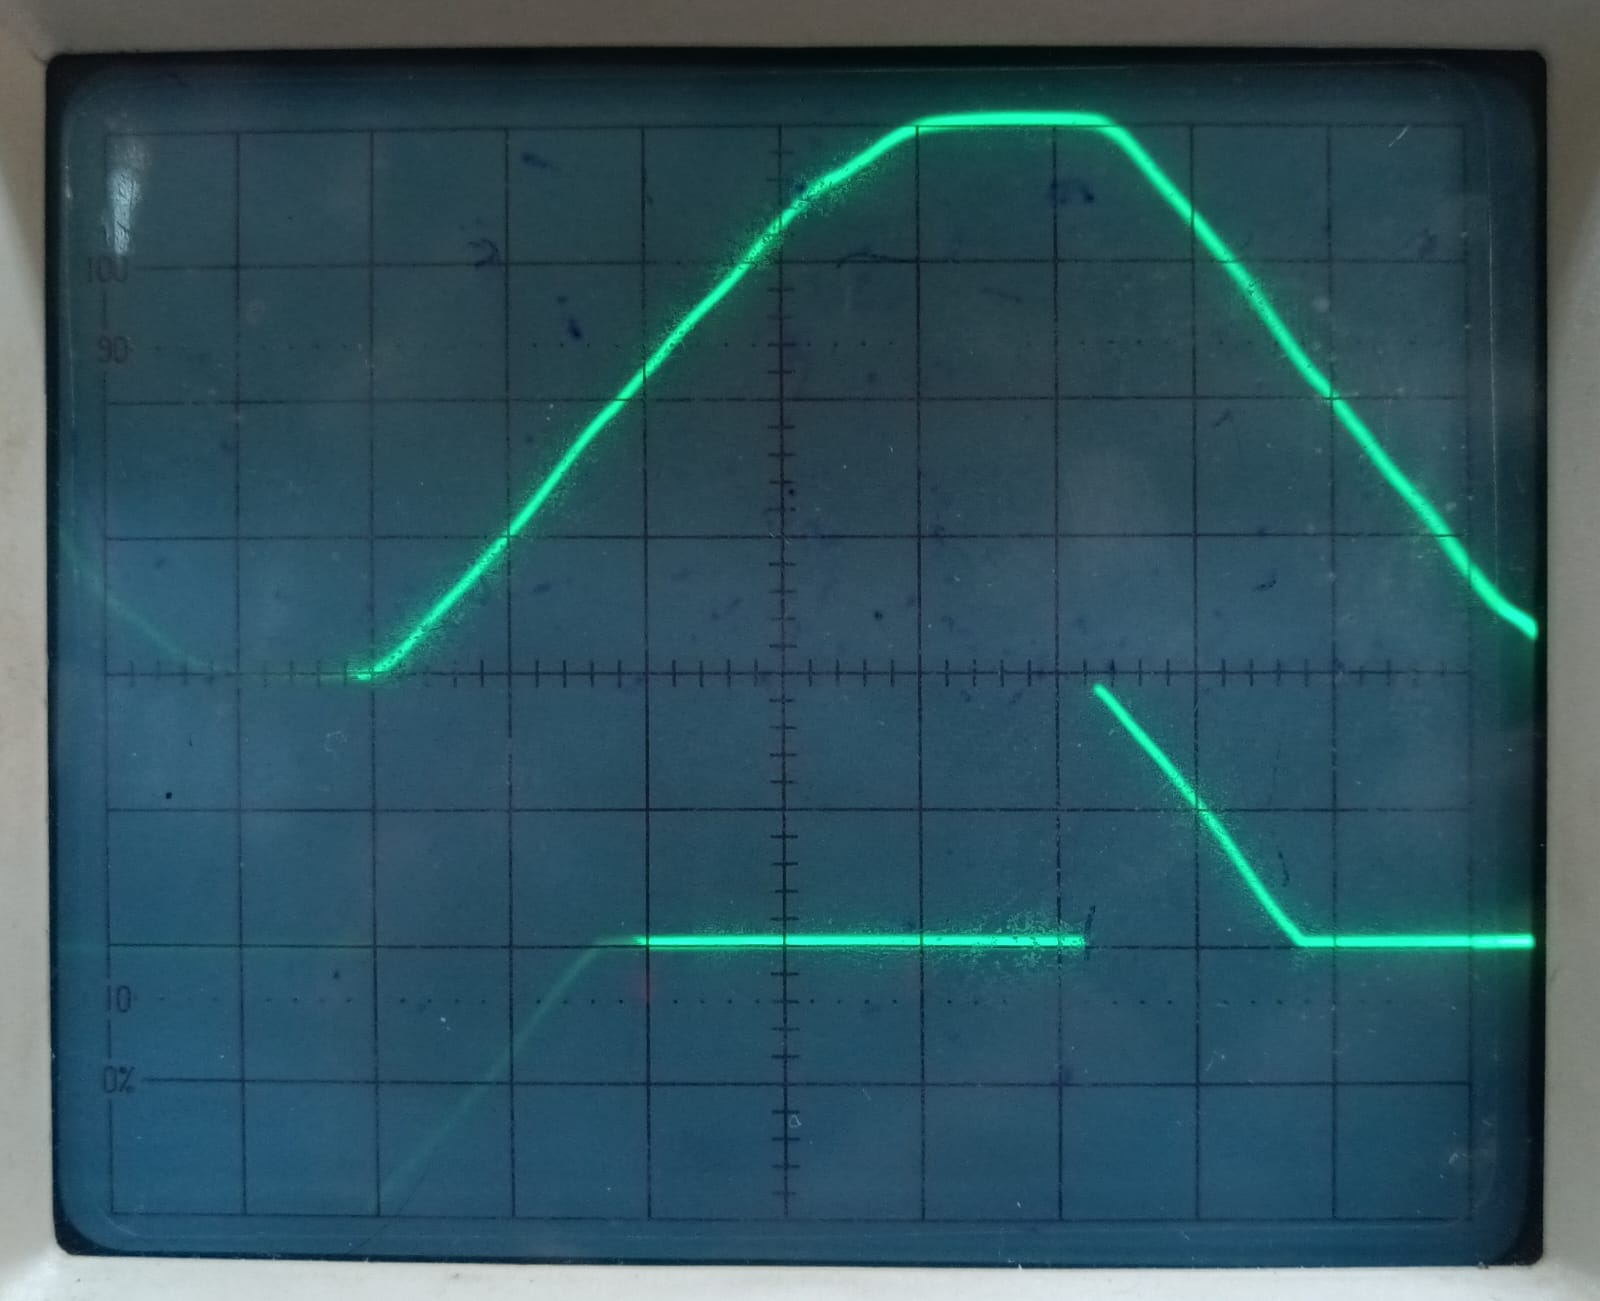
\includegraphics[width=0.65\textwidth]{Imagenes/60grad.jpeg}
        \label{}
        \caption{$Ang_{cond}=60$°}
    \end{subfigure}
    \hfill
        \begin{subfigure}[b]{0.49\textwidth}
        \centering  
            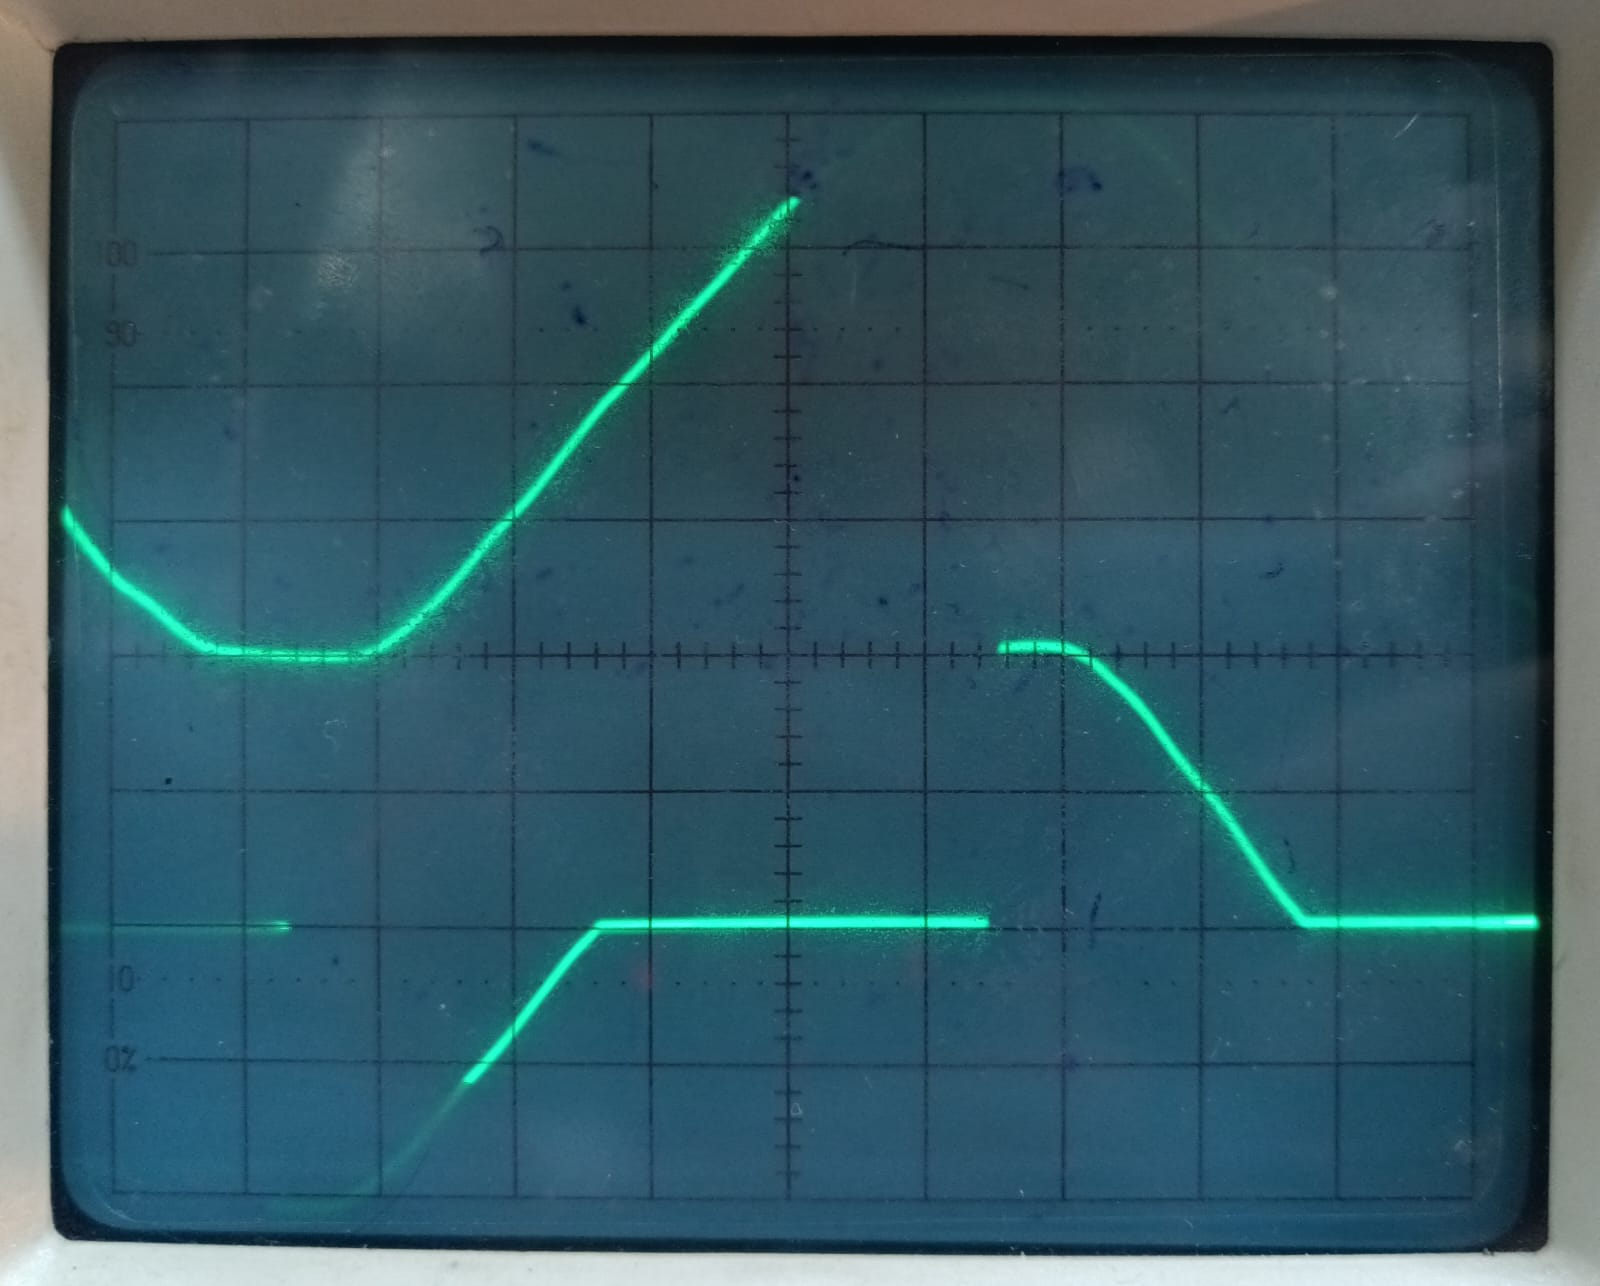
\includegraphics[width=0.65\textwidth]{Imagenes/90grad.jpeg}
        \label{}
        \caption{$Ang_{cond}=90$°}
    \end{subfigure}
    \hfill
        \begin{subfigure}[b]{0.5\textwidth}
        \centering  
            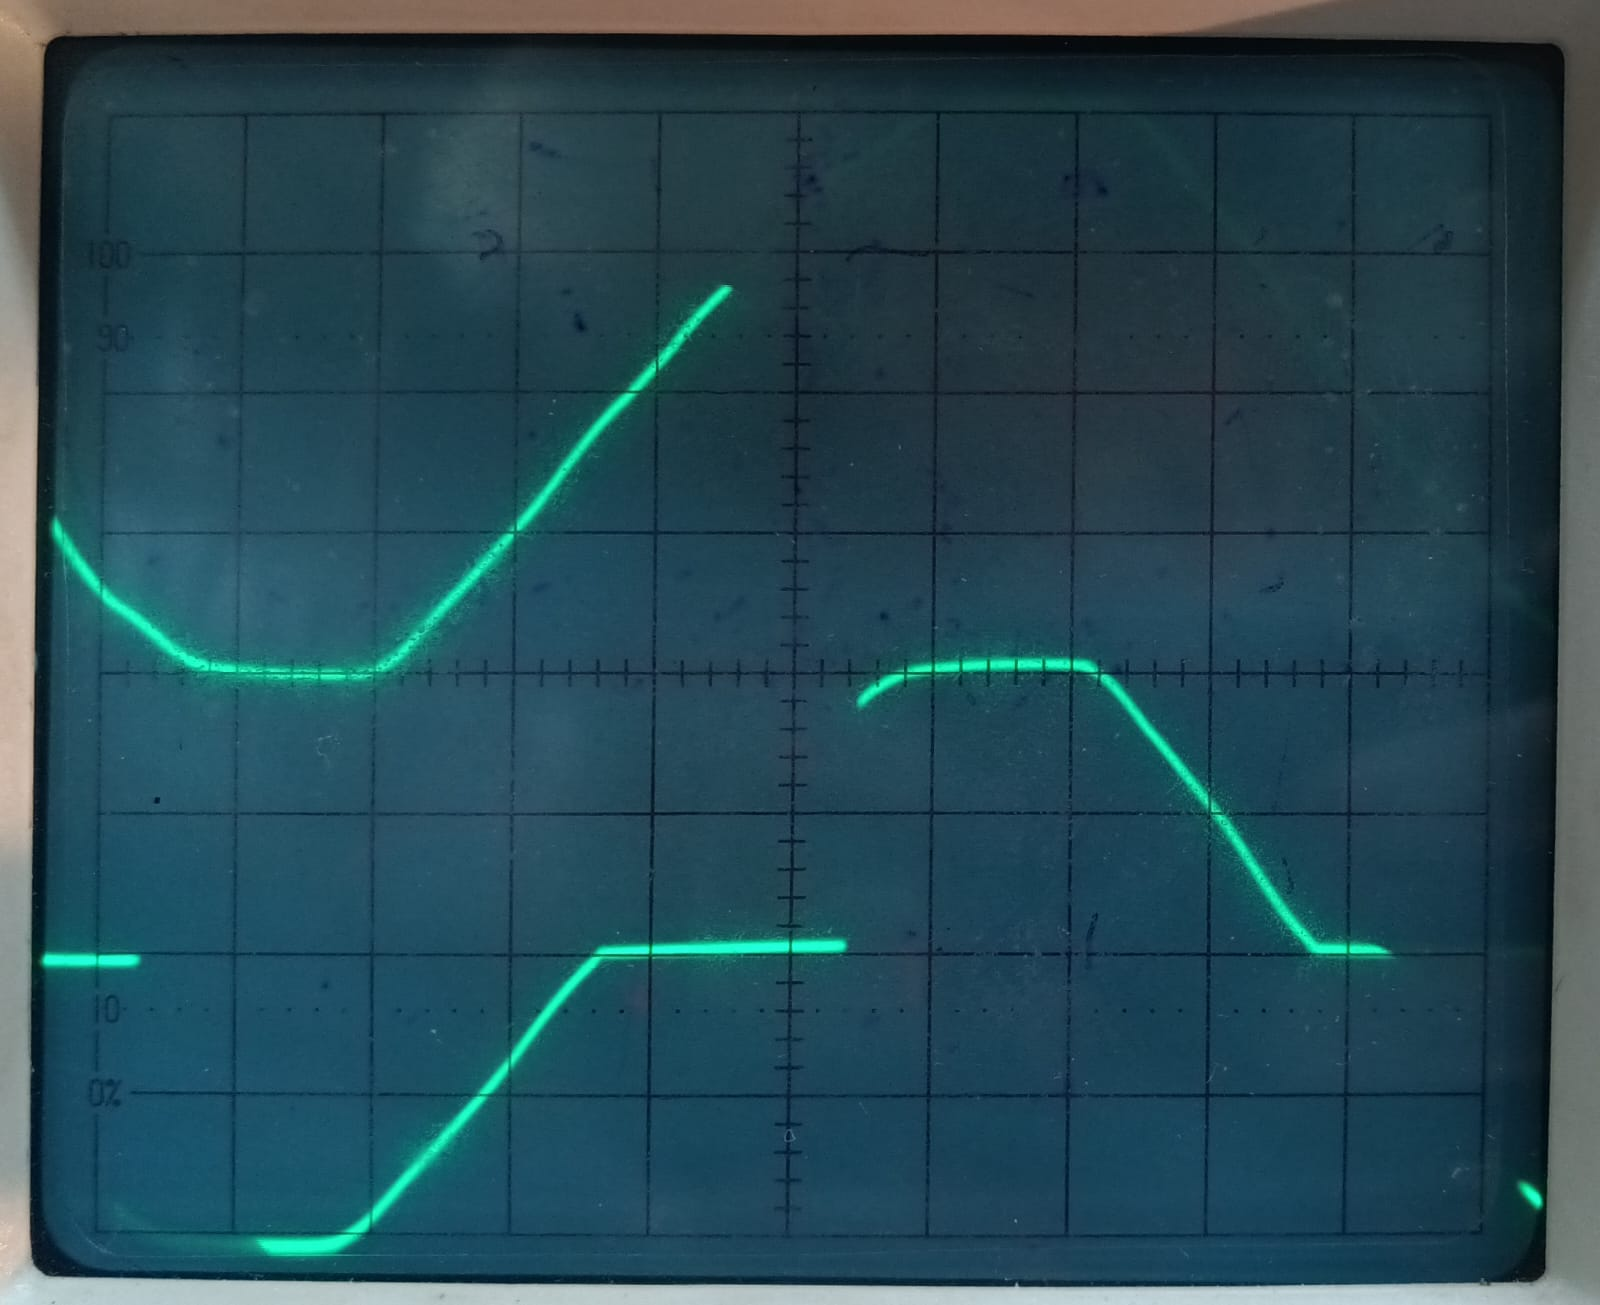
\includegraphics[width=0.65\textwidth]{Imagenes/120grad.jpeg}
        \label{}
        \caption{$Ang_{cond}=120$°}
    \end{subfigure}
    \hfill
        \begin{subfigure}[b]{0.49\textwidth}
        \centering  
            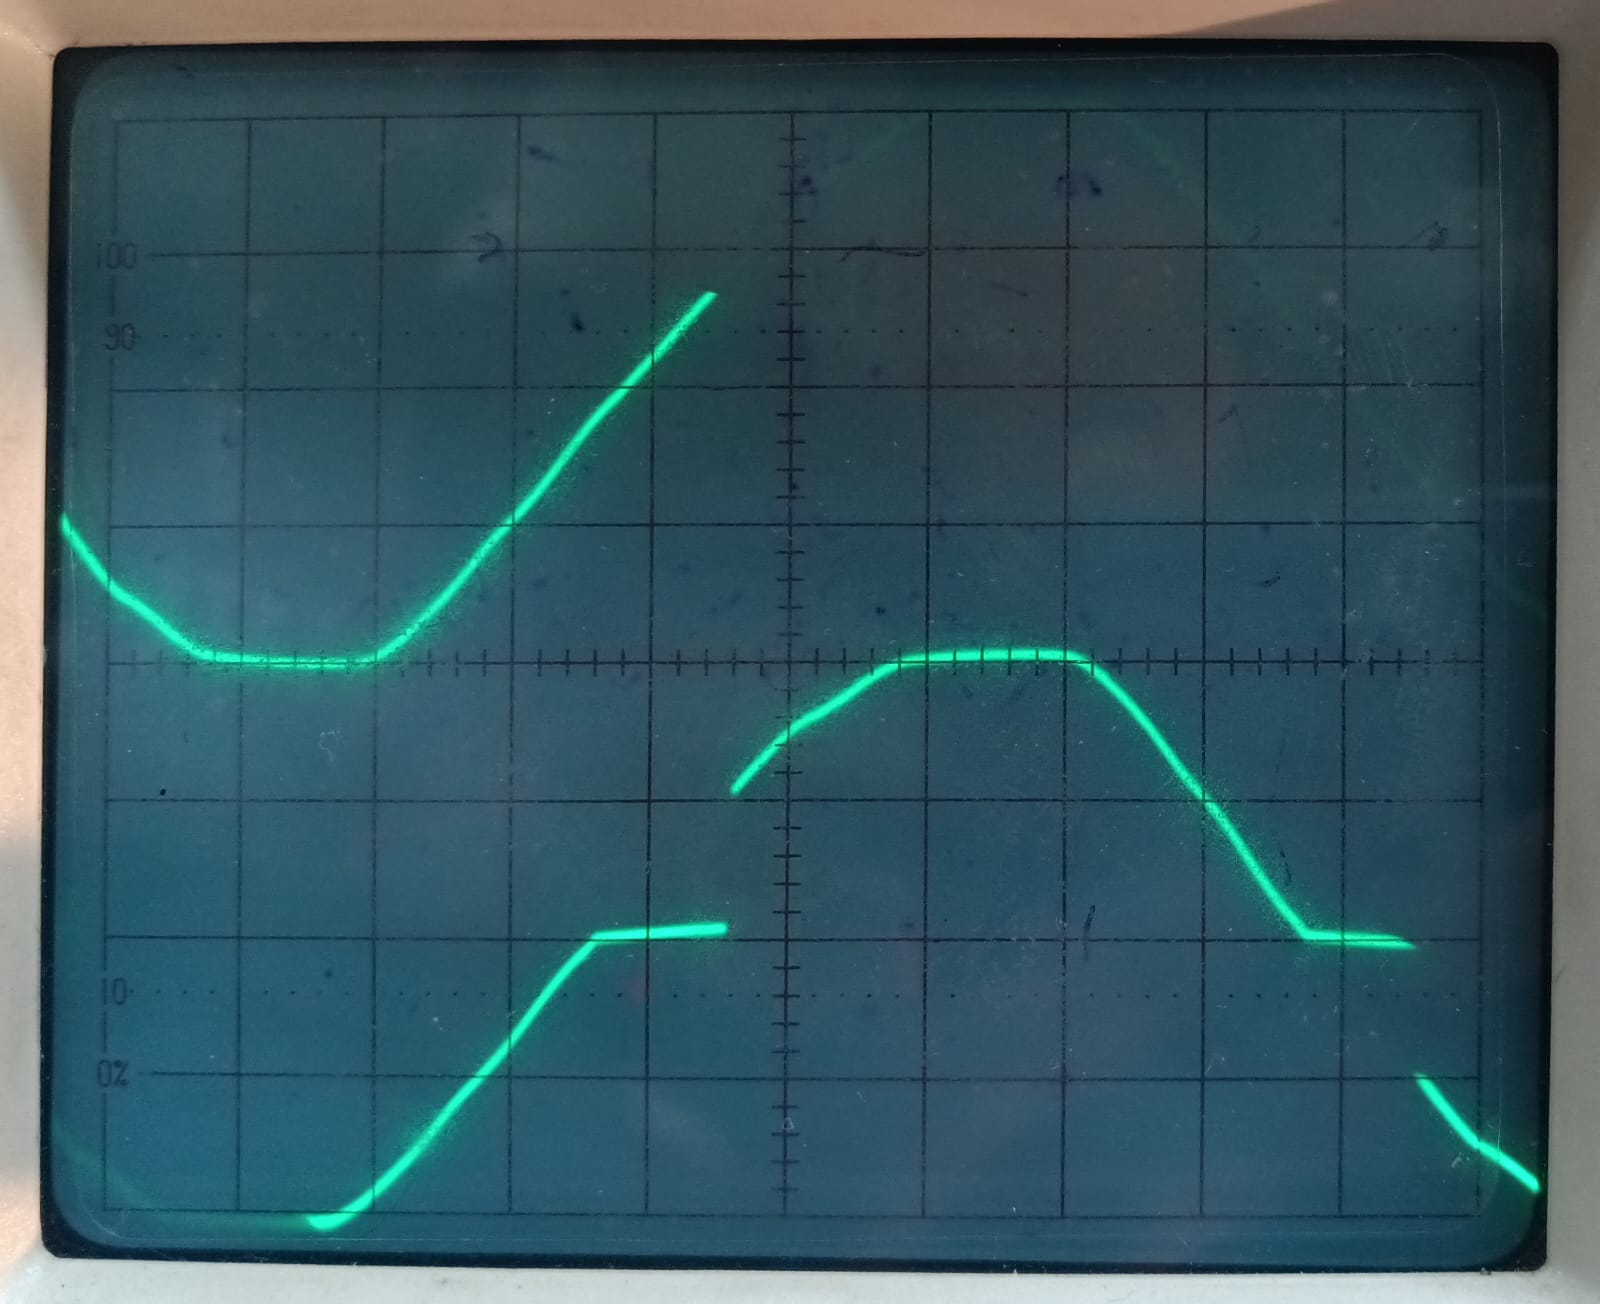
\includegraphics[width=0.65\textwidth]{Imagenes/150grad.jpeg}
        \label{}
        \caption{$Ang_{cond}=150$°}
    \end{subfigure}
    \caption{Señales con diferentes ángulos de conducción}
    \label{fig:fot_exp4}
    \end{center}
\end{figure}



Se pudo observar que el valor medido por el multimetro de respuesta al valor medio se aproxima al medido por el multimetro \textit{TrueRMS} a medida que la señal $V_o$ se aproxima a una señal sinusoidal. 

\unsubsubsection{Gráficos}

\begin{figure}[H]
    \centering
    \begin{tikzpicture}[scale=1]
        \coordinate (a1) at (0,0);
        \coordinate (a2) at (2,0.186*4);
        \coordinate (a3) at (4,0.386*4);
        \coordinate (a4) at (6,0.503*4);
        \coordinate (a5) at (8,0.906*4);
        \coordinate (a6) at (10,0.984*4);
        \coordinate (a7) at (12,1*4);

    \draw[thin,gray!40] (0,0) grid (12,4);
    \draw[<->] (0,0)--(12,0) node[right] {$[^\circ]$};
    \draw[<->] (0,0)--(0,4) node[above]{$\frac{V_o}{V_i}$};


    \foreach \a [evaluate={\y=int(\a*15)}] in {0,2,...,12}{
        \draw[line width=0.7pt,dotted] (\a,0) node[below]{\footnotesize $\y^\circ$};
    }
    \foreach \a [evaluate={\y=(\a*0.25)}] in {0,1,...,4}{
        \draw[line width=0.7pt,dotted] (0,\a) node[left]{\footnotesize $\y$};
    }
    \foreach \a in{1,...,7}{
       \draw[thin,dashed,black] let \p1=(a\a) in (\x1,0)--(a\a);
       \draw[line width=1pt,black](a\a) circle(1pt);
    }
    \foreach \x [evaluate={\y=int(\x+1);}] in {1,...,6}{
        \draw[line width=1pt,black] (a\x) -- (a\y);
   }
    
\end{tikzpicture}
\caption*{$V_o$ medido por el multimetro \textit{TrueRMS}}
    \begin{tikzpicture}[scale=1]
        \coordinate (a1) at (0,0);
        \coordinate (a2) at (2,0.074*4);
        \coordinate (a3) at (4,0.204*4);
        \coordinate (a4) at (6,0.295*4);
        \coordinate (a5) at (8,0.767*4);
        \coordinate (a6) at (10,0.931*4);
        \coordinate (a7) at (12,1*4);

    \draw[thin,gray!40] (0,0) grid (12,4);
    \draw[<->] (0,0)--(12,0) node[right] {$[^\circ]$};
    \draw[<->] (0,0)--(0,4) node[above]{$\frac{V_o}{V_i}$};


    \foreach \a [evaluate={\y=int(\a*15)}] in {0,2,...,12}{
        \draw[line width=0.7pt,dotted] (\a,0) node[below]{\footnotesize $\y^\circ$};
    }
    \foreach \a [evaluate={\y=(\a*0.25)}] in {0,1,...,4}{
        \draw[line width=0.7pt,dotted] (0,\a) node[left]{\footnotesize $\y$};
    }
    \foreach \a in{1,...,7}{
       \draw[thin,dashed,black] let \p1=(a\a) in (\x1,0)--(a\a);
       \draw[line width=1pt,black](a\a) circle(1pt);
    }
    \foreach \x [evaluate={\y=int(\x+1);}] in {1,...,6}{
        \draw[line width=1pt,black] (a\x) -- (a\y);
   }
    
\end{tikzpicture}
\caption*{$V_o$ medido por el multimetro con respuesta $V_{media}$}
   % \begin{tikzpicture}[scale=1]
\def\scal{1.5}
        \coordinate (a1) at (0,0);
        \coordinate (a2) at (2,1.52*\scal);
        \coordinate (a3) at (4,0.89*\scal);
        \coordinate (a4) at (6,0.7*\scal);
        \coordinate (a5) at (8,0.18*\scal);
        \coordinate (a6) at (10,0.05*\scal);
        \coordinate (a7) at (12,0);

    \draw[thin,gray!40,ystep=\scal] (0,0) grid (12,4);
    \draw[<->] (0,0)--(12,0) node[right] {$[^\circ]$};
    \draw[<->] (0,0)--(0,4) node[above]{$\kappa$};


    \foreach \a [evaluate={\y=int(\a*15)}] in {0,2,...,12}{
        \draw[line width=0.7pt,dotted] (\a,0) node[below]{\footnotesize $\y^\circ$};
    }
    \foreach \a [evaluate={\y=int(\a+1)}] in {0,1,...,2}{
        \draw[line width=0.7pt,dotted] (0,\a*\scal) node[left]{\footnotesize $\y$};
    }
    \foreach \a in{1,...,7}{
       \draw[thin,dashed,black] let \p1=(a\a) in (\x1,0)--(a\a);
       \draw[line width=1pt,black](a\a) circle(1pt);
    }
    \foreach \x [evaluate={\y=int(\x+1);}] in {1,...,6}{
        \draw[line width=1pt,black] (a\x) -- (a\y);
   }
    
\end{tikzpicture}
\caption*{Factor de corrección $\kappa=\frac{V_{TRms}}{V_{MRms}}$ }
    \label{fig:vivo}
\end{figure}

\unsubsubsection{Factor de Corrección}

\begin{figure}[H]
    \centering
    \begin{tikzpicture}[scale=1]
\def\scal{1.5}
        \coordinate (a1) at (0,0);
        \coordinate (a2) at (2,1.52*\scal);
        \coordinate (a3) at (4,0.89*\scal);
        \coordinate (a4) at (6,0.7*\scal);
        \coordinate (a5) at (8,0.18*\scal);
        \coordinate (a6) at (10,0.05*\scal);
        \coordinate (a7) at (12,0);

    \draw[thin,gray!40,ystep=\scal] (0,0) grid (12,4);
    \draw[<->] (0,0)--(12,0) node[right] {$[^\circ]$};
    \draw[<->] (0,0)--(0,4) node[above]{$\kappa$};


    \foreach \a [evaluate={\y=int(\a*15)}] in {0,2,...,12}{
        \draw[line width=0.7pt,dotted] (\a,0) node[below]{\footnotesize $\y^\circ$};
    }
    \foreach \a [evaluate={\y=int(\a+1)}] in {0,1,...,2}{
        \draw[line width=0.7pt,dotted] (0,\a*\scal) node[left]{\footnotesize $\y$};
    }
    \foreach \a in{1,...,7}{
       \draw[thin,dashed,black] let \p1=(a\a) in (\x1,0)--(a\a);
       \draw[line width=1pt,black](a\a) circle(1pt);
    }
    \foreach \x [evaluate={\y=int(\x+1);}] in {1,...,6}{
        \draw[line width=1pt,black] (a\x) -- (a\y);
   }
    
\end{tikzpicture}
\caption*{Factor de corrección $\kappa=\frac{V_{TRms}}{V_{MRms}}$ }
\end{figure}

